\documentclass[border=0bp]{standalone}
\usepackage[T1]{fontenc}
\usepackage{newpxtext,newpxmath,graphicx,tikz}
\definecolor{retained}{HTML}{D8EAE8}
\definecolor{ink}{HTML}{205C5B}
\definecolor{diagonal}{HTML}{F2E6D5}
\begin{document}
\begin{tikzpicture}[x=1bp,y=-1bp,font=\fontsize{17bp}{20bp}\selectfont]
\path[use as bounding box] (0,0) rectangle (859,526);
\node[anchor=west,font=\bfseries\fontsize{18bp}{21bp}\selectfont] at (8,15) {(a) The normalized half-triangle};
\node[anchor=east] at (30,45) {$n$};
\draw[gray!55,dashed] (286,34) -- (286,222);
\foreach \n in {0,...,7} {
  \pgfmathsetmacro{\yy}{45+22*\n}
  \node[anchor=east,text=gray!75!black] at (62,\yy) {$\n$};
  \foreach \k in {0,...,\n} {
    \pgfmathsetmacro{\xx}{286+48*(\k-\n/2)}
    \pgfmathtruncatemacro{\value}{round(factorial(\n)/(factorial(\k)*factorial(\n-\k)))}
    \def\shade{white}\def\numcolor{gray!75!black}
    \ifnum\k=0 \def\shade{gray!13}\fi
    \ifnum\k=\n \def\shade{gray!13}\fi
    \ifnum\n>1 \ifnum\k=1 \def\shade{diagonal}\fi\fi
    \ifnum\k>1
      \pgfmathtruncatemacro{\twok}{2*\k}
      \ifnum\twok>\n\else\def\shade{retained}\def\numcolor{ink}\fi
    \fi
    \node[fill=\shade,text=\numcolor,rounded corners=3bp,minimum width=34bp,minimum height=20bp,inner sep=0pt] at (\xx,\yy) {$\value$};
  }
}
\node[anchor=east] at (94,225) {$k=$};
\foreach \k in {0,...,7} {
  \pgfmathsetmacro{\xx}{118+48*\k}
  \node[text=gray!75!black] at (\xx,225) {$\k$};
}
\draw[<->,ink,thick] (214,249) -- (358,249);
\node[fill=white,inner sep=3bp,text=ink] at (286,249) {$k\leftrightarrow n-k$};
\node[anchor=north west,inner sep=0pt,text width=300bp,align=left] at (537,42) {Position $k$ in row $n$ contains $\binom nk$.};
\node[anchor=west,fill=gray!13,rounded corners=3bp,inner sep=5bp] at (537,105) {Boundary: $k=0,n$, all ones};
\node[anchor=west,fill=diagonal,rounded corners=3bp,inner sep=5bp] at (537,143) {Omit the diagonal $k=1$};
\node[anchor=west,fill=retained,text=ink,rounded corners=3bp,inner sep=5bp] at (537,181) {Retain $2\leq k\leq n/2$};
\node[anchor=north west,inner sep=0pt,text width=298bp,align=left] at (537,216) {Reflection pairs equal entries. Keep a central entry only once.};
\node[anchor=west,font=\bfseries\fontsize{18bp}{21bp}\selectfont] at (8,281) {(b) The neighboring occurrences of $3003$};
\begin{scope}[shift={(0,293)}]
\node[anchor=north west,inner sep=0pt] at (0,0) {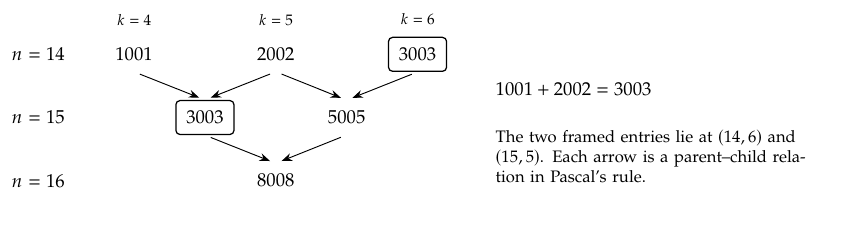
\includegraphics[width=859bp,height=233bp]{fig01_pascal_original.png}};
\fill[white] (490,122) rectangle (857,232);
\node[anchor=north west,inner sep=0pt,text width=346bp,align=left,font=\fontsize{17bp}{20bp}\selectfont] at (495,130) {The two framed entries lie at $(14,6)$ and $(15,5)$. Each arrow joins an entry to an entry in the next row to which it contributes.};
\end{scope}
\end{tikzpicture}
\end{document}
